\chapter{Desarrollo de la aplicación.}

\section{Desarrollo Web.}

A continuación se describe detalladamente el proceso de construcción que se utilizó para el desarrollo de la aplicación web, seguiendo el estándar de \emph{Rails}, se adoptó una metodología ágil\footnote{Es un proceso de desarrollo de software, desarrollado inicialmente por James Martin en 1980. El método comprende el desarrollo iterativo, y la construcción de prototipos, tiende a englobar también la usabilidad, utilidad y la rapidez de ejecución.} buscando velocidad en el desarrollo del producto, así como calidad, pues la aplicación supliría las necesidades de los usuarios y se entregaría en un tiempo acorde según los límites de tiempo del proyecto.

\subsection{Especificaciones.}

El primer paso para desarrollar apropiadamente una aplicación guiada por tests(\emph{Test Driven Development - TDD}), es definir las especificaciones que determinan el comportamiento del sistema, dichas especificaciones más tarde se convertirán en la base de los tests para el desarrollo de la aplicación.\\

En este punto, se describió la aplicación Web a ser escrita teniendo en cuenta la definición del problema y el marco referencial, la tarea principal entonces sería integrar datos con contenidos para lograr el desarrollo final de la aplicación, después de tener claro la necesidad a cubrir y de que se necesitaba brindar un ambiente de fácil acceso y manipulación para los usuarios, se decidió desarrollar una aplicación web con las siguientes especificaciones(especificaciones que mas tarde se ampliarían para la construcción de los test.):


\begin{itemize}
\item[$\bullet$] Sistema de usuarios protegido por contraseña.
\item[$\bullet$] Cada usuario puede registrar un portafolio.
\item[$\bullet$] Cada portafolio esta compuesto por títulos.
\item[$\bullet$] Los títulos representan el estado personal de una acción registrada por el usuario, para de esa manera determinar, si la inversión le representa a su propietario una perdida o una ganancia.
\item[$\bullet$] Dentro del portafolio se pueden agregar, actualizar, comparar y eliminar títulos.
\item[$\bullet$] Cada título puede ser seleccionado para inspeccionar su comportamiento durante un rango de tiempo determinado por el usuario.
\item[$\bullet$] Los títulos de cada usuario pueden ser comparados simultáneamente con el apoyo de los contenidos 3D.
\item[$\bullet$] Los títulos se basan en la información que se obtiene al actualizar las acciones.
\item[$\bullet$] Las acciones se actualizan cada veinte minutos cuándo el mercado esta abierto.
\item[$\bullet$] La página principal no necesita registro, evidencia el comportamiento del mercado con una gráfica en 3D y muestra el estado actual de cada acción.
\end{itemize}

\subsection{Definición de modelos.}

Con el comportamiento de la aplicación claro, era necesario entonces definir los datos con los que la misma trabajaría, que tablas se necesitarían, que campos, y que tipos de datos estarían siendo manipulados por la aplicación, y cuáles  alimentarían los contenidos 3D.\\

Aparte de los definición de los modelos involucrados, se buscaba estar en la capacidad de trabajar bajo un patrón \textbf{ActiveRecord}\footnote{Es un enfoque al problema de acceder a los datos de una base de datos. Una fila en la tabla de la base de datos se envuelve en una clase, de manera que se asocian filas únicas de la base de datos con objetos del lenguaje de programación usado. Cuando se crea uno de estos objetos, se añade una fila a la tabla de la base de datos. Cuando se modifican los atributos del objeto, se actualiza la fila de la base de datos. La clase envoltorio implementa métodos de acceso para cada columna de la tabla o vista.} pensando en un enfoque \textbf{ORM}\footnote{Léase \textbf{ORM} en el glosario.} que permitiera manipular los registros de la base datos como si se trataran de objetos definidos en el lenguaje de programación \emph{Ruby}.\\

El modelo entidad relación final, y que representa la estructura de la base de datos de la aplicación es el que se muestra en la Figura \ref{fig:erd}, según la información recogida de las especificaciones, era claro que se necesitaba un modelo que representara los usuarios, a su vez dichos usuarios tienen relacionado un portafolio(relación \emph{1..1}), cada portafolio actúa como contenedor de títulos(relación \emph{1..n}), indirectamente entonces, el usuario posee títulos, como sucede en la vida real, el modelo \emph{stock\_action} representa la acción real en el mercado, y sobre la cual existen múltiples títulos asociados.

\begin{figure}[h]
	\centering
		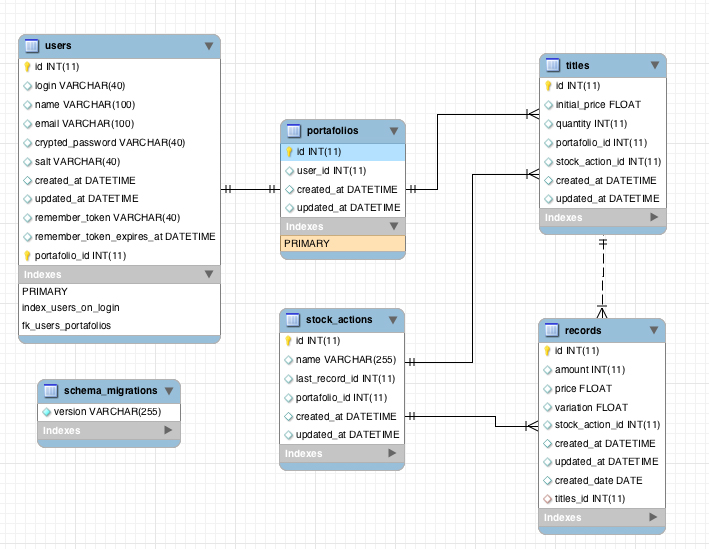
\includegraphics[scale=0.4]{erb_mertd.jpg}
		\caption{Modelo Entidad Relación - Mertd(Mercado 3D)}
	\label{fig:erd}
\end{figure}

Finalmente el modelo \emph{record} es sobre el cual se registran todos los movimientos de las acciones, es decir, sobre el que se hacen las actualizaciones según el estado de una acción, por ejemplo, cada vez que se obtiene información nueva indicando el estado de una acción, un registro nuevo es agregado y guardado en este modelo, luego este registro es usado por otros modelos para calcular el estado de una inversión de forma personalizada.\\

La siguiente porción de código de la aplicación, muestra claramente cómo se puede sacar provecho al utilizar un patrón como \textbf{ActiveRecord}, según este patrón, si existe una tabla \emph{titles} debe haber una clase \emph{Title} asociada, sobre la cual se hace el mapeo.

\begin{verbatim}
	t = Title.new
	t.initial_price = 15250.66
	t.quantity = 10000
	t.portafolio = p #p es un portafolio existente cuya id es 1
	t.stock_action = s_a #s_a es una acción existente cuya id es 15
	t.save
	#otra manera mas corta de hacer este regristro, podría ser:
	#t = Title.new(:initial_price => 15250.66, :quantity => 10000, 
	#			   :portafolio => p, :stock_action => s_a)
	#
\end{verbatim}

A nivel de bases de datos, las anteriores declaraciones son interpretadas de la siguiente manera:

\begin{verbatim}
INSERT INTO titles 
  (initial_price, quantity, portafolio_id, stock_action_id) 
  VALUES (15250.66, 10000, 1, 15);
\end{verbatim}

Cabe resaltar que siempre será más rápido ejecutar directamente el código nativo interpretado por el motor de base de datos, pero en éste caso se opto por la claridad de código y la manipulación de objetos pues no se requirió diseñar consultas que hicieran que la diferencia de tiempos entre uno y otro método fuera considerable.

\subsection{Configuración.}
\subsection{Ambientes.}
\subsection{Daemon - \emph{Stock Getter}.}
\subsection{\emph{TDD Cycle}}

\section{Desarrollo Contenidos 3D}
La arquitectura dentro de una escena en Unity3D consiste en un conjunto de GameObjects que interactúan entre si para mostrar un evento/animación en una escena; Dichos objetos interactúan entre si, basándose en una jerarquía de objetos, donde la traslación/rotación/escalamiento de un padre afecta directamente a los hijos.

ACA MOSTRAR LA INTERFAZ DE UNITY CON LOS PADRES / HIJOS

Se decidió entonces dividir el programa en 3 grandes modulos.
ACA VA IMAGEN GRILLA DE LOS MODUlOS
\subsection{Módulo de detección de datos de información del exterior:}

\subsection{Módulo de renderizado de escena(Grapher):}

\subsection{Modulo de información de Objetos:}



Basicamente 4 tipos de gráficos fueron los que se decidieron desarrollar y fueron: Barras, Espiral, Superficie y el `Campo'. cada gráfica ofrece información relevante para cada tipo de variable que se esta analizando. 

Barras: Son las típicas barras que se pueden encontrar en cualquier visualizacion de acciones, pero con el valor agregado de que permiten ver el comportamiento de una o varias acciones a través del tiempo.

Espiral: Este tipo de gráfica permite comparar rendimientos de varias acciones por medio del porcentaje de variación de cada una en un momento determinado, es el único tipo de grafico que no permite comparar acciones a través del tiempo, pues lo único que interesa en este gráfico, es determinar de una manera fácil y rápida que acciones estan generando mas rentabilidad, cuales estan perdiendo y cuales estan invariantes en un tiempo determinado.

Superficie: Este tipo de gráfico también compara rentabilidades de dos o mas acciones a través del tiempo con respecto a la mayor/menor  rentabilidad de todas las acciones en un momento determinado  y va generando una superficie 3D que describe el comportamiento de la bolsa a travez de un periodo de tiempo.

Campo: Es el tipo de gráfico mas complejo que se realizó, pues en este gráfico comparamos variables de cantidad Vs Rentabilidad a travez del tiempo, entonces a través de estas variables podemos inferir si una accion se esta tranzando en la bolsa en mucha cantidad o no y si dicha acción esta siendo rentable; Este grafico provee una serie de "Zonas" que ayudan al usuario a determinar las acciones en que estado se encuentran en un momento determinado, y asi inferir facilmente si la acción esta generando perdidas o ganancias.

 

\section{Desarrollo protocolo de comunicación.}

\section{Deployment}

\section{SCM}